\documentclass[a4paper]{scrreprt}

\usepackage{tikz}
\usetikzlibrary{positioning,calc}

\usepackage{lmodern}
\usepackage{microtype}
\usepackage[utf8]{inputenc}
\usepackage[T1]{fontenc}

\usepackage{amsmath}
\usepackage{amssymb}
\usepackage{amsfonts}
\usepackage[amsmath,amsthm,thref]{ntheorem}
\usepackage[retainorgcmds]{IEEEtrantools}

\usepackage{makeidx}
\usepackage{booktabs}
\usepackage{array}
\usepackage{float}
\usepackage{xfrac}

\title{Galois Theory}
\author{Wenda Zhou}

\newcommand\restr[2]{{% we make the whole thing an ordinary symbol
  \left.\kern-\nulldelimiterspace % automatically resize the bar with \right
  #1 % the function
  \vphantom{\big|} % pretend it's a little taller at normal size
  \right|_{#2} % this is the delimiter
  }}

\newcommand{\homset}[3][K]{
  \ensuremath{\text{Hom}_{#1}\left(#2, #3\right)}
}

\newcommand{\rootset}[2][P]{
  \ensuremath{\text{Root}_{#1}\left(#2\right)}
}

\newcommand{\autset}[2][K]{\ensuremath{\text{Aut}_{#1}\left(#2\right)}}

\newcommand{\cardinality}[1]{
  \ensuremath{\left|#1\right|}
}

\newcommand{\card}[1]{\cardinality{#1}}

\newcommand{\Gal}[1]{\ensuremath{\text{Gal}\left(#1\right)}}

\newcommand{\multCyclicGp}[1]{\ensuremath{\left(\sfrac{\mathbb{Z}}{(#1)}\right)^{\times}}}
\newcommand{\unityroots}[1]{\ensuremath{\mathbf{\mu}_{#1}}}

\newcommand{\finitefield}[1]{\ensuremath{\mathbb{F}_{#1}}}

\DeclareMathOperator{\mchar}{char}

%%% Local Variables: 
%%% mode: latex
%%% TeX-master: "Galois"
%%% End: 

\declaretheorem{theorem}
\declaretheorem[sibling=theorem]{lemma}
\declaretheorem[sibling=theorem]{proposition}
\declaretheorem[sibling=theorem]{corollary}
\declaretheorem[sibling=theorem]{definition}


%%% Local Variables: 
%%% mode: latex
%%% TeX-master: "Galois"
%%% End: 


\newcolumntype{V}{>{\centering\arraybackslash} m{0.4\linewidth}}

\makeindex

\begin{document}

\maketitle


\section{Complex differentiation}
\label{sec:1}

Recall the following:
\begin{itemize}
\item  $U \subseteq \CC$ is open\index{open} if $\forall x \in U, \exists \epsilon > 0 \text{ such that } B_\epsilon(x) = \{ y | \abs{y-x} < \epsilon \}  \subseteq U$.
\item $U$ is path-connected\index{path-connected} of $\forall x, y \in U, \exists \gamma : [0, 1] \rightarrow U, \gamma \text{ continuous }, \gamma(0) = x, \gamma(1) = y$.
\end{itemize}

\begin{definition}
  We say that a function $f : U \rightarrow \CC$ on an open set $U \in \CC$ is differentiable\index{differentiable} at $< \in U$ if:
\[
\lim_{z\rightarrow w} \frac{f(z) - f(w)}{z - w}
\]
exists. If so, we call this limit $f'(w)$.

 We say that $f$ is holomorphic\index{holomorphic} at $w \in U$ if $\exists \epsilon > 0$ such that $f$ is differentiable on $B_\epsilon(w) \subseteq U$.
\end{definition}

\begin{definition}
  An entire\index{entire} function $f : \CC \rightarrow \CC$ is one that is holomorphic on $\CC$.
\end{definition}

\begin{remark}
  Sum and product rules, rules for differentiating inverses etc. carry over to complex differentiable functions.
\end{remark}

Tautologically, a function $f : U \rightarrow \CC$ can be written $f = u(x, y) + iv(x, y)$ for functions $u, v : \RR^2 \rightarrow \RR$. Recall that $u : U \rightarrow \RR$ (as a function of 2 real variables) is differentiable at $(c, d)$ with derivative $\mathrm{D}u_{(c, d)} = (\lambda, \mu)$ if:
\[
\frac{u(x, y) - u(c, d) - \left(\lambda(x - c) + \mu(y - d)\right)}{\norm{(x, y) - (c, d)}} \rightarrow 0 \text{ as } (x, y) \rightarrow (c, d)\mpunct{.}
\]

\begin{proposition}
  Let $f(z) = u(x, y) + iv(x, y)$ be defined on an open $U \subseteq \CC$. Let $z = c+id \in U$. Then $f$ is differentiable at $z$ if and only if:
  \begin{itemize}
  \item $e$, $v$ are differentiable at $(c, d)$ and
  \item $u_x = v_y$ and $u_y = -v_x$ at $(c, d)$ (Cauchy-Riemann equations\index{Cauchy-Riemann equations}.
  \end{itemize}
In this cases, we have that $f'(z) = u_x(c, d) + iv_x(c, d)$.
\end{proposition}

\begin{proof}
  $f$ is differentiable at $w$ with derivative $f'(w) = p + iq$, $p, q \in \RR$, if and only if:
\[
\lim_{z\rightarrow w} \frac{f(z) - f(w) - f'(w)(z-w)}{\abs{z - w}} = 0\mpunct{.}
\]
Taking real and imaginary parts (putting $z = x + iy$, $w = c + id$ for $x, y, c, d, \in \RR$) and using the fact that $f'(w) =  + iq$, then we have:
\[
f'(w)(z-w) = p(x-c) - q (x - c) + i\left(q(x-c) + p(y-d)\right)\mpunct{.}
\]
The previous limit is zero if and only if:
\[
\lim_{(x, y) \rightarrow (c, d)} \frac{u(x, y) - u(c, d) - \left(p(x - c) - q(y - d)\right)}{\sqrt{(x-c)^2 + (y-d)^2}} = 0
\]
and
\[
\lim_{(x, y) \rightarrow (c, d)} \frac{v(x, y) - v(c, d) - \left(q(x-c) + p(y-d)\right)}{\sqrt{(x-c)^2 + (y-d)^2}} = 0\mpunct{.}
\]
Comparing to the definition of differentiability of $u, v : \RR^2 \rightarrow \RR$ yields that $u$, $v$ are differentiable at $(c, d)$ and:
\[
\mathrm{D}u_{(c, d)} = (p, -q) \text{ and } \mathrm{D}v_{(c, d)} = (q, p)
\]
which are the Cauchy-Riemann equations.
\end{proof}

\emph{Warning}: if $f = u + iv$, and $u_x = v_y$ and $u_y = -v_x$ hold at a point $w$, it doesn't follow that $f$ is differentiable at $w$ (see example sheet 1). To conclude that $f$ is differentiable, we need to have that $u$, $v$ are differentiable and not just that their partial derivatives exist.

\begin{remark}
  To see $f$ differentiable at $w$ implies that $u$, $v$ have partial derivatives satisfying the Cauchy-Riemann equations, consider:
  \begin{IEEEeqnarray*}{rCl}
    f'(w) &=& \lim_{\substack{h\rightarrow 0 \\ h \in \RR}} \frac{f(w + h) - f(w)}{h} \\
    &=& \lim_{\substack{h\rightarrow 0 \\ h \in \RR_+}} \frac{u(c + h, d) - u(c, d)}{h} + i \frac{v(c+h, d) - v(c, d)}{h} \\
    &=& u_x(c, d) + iv_x(c, d)\mpunct{.}
  \end{IEEEeqnarray*}
We can obtain a similar expression for the second Cauchy-Riemann equation taking $z \rightarrow w$ via $w + ih$, $h \rightarrow 0$.
\end{remark}

\paragraph{Examples}

\begin{itemize}
\item Any polynomial $p : \CC \rightarrow \CC$ defines an entire function.
\item A ration $p/q$ of complex polynomials defines a function holomorphic on $\CC \setminus \{ \text{zeroes} (q) \}$.
\item Further examples via power series.
\item $f(z) = \abs{z}$ is not differentiable at any point of $\CC$. Let $f(z) = u(x, y) + iv(x, y)$, where $u(x, y) = \sqrt{x^2 + y^2}$ and $v = 0$. So $v_x = v_y = 0$. Away from $(x, y) = (0, 0)$, we have that:
\[
u_x = \frac{x}{\sqrt{x^2 + y^2}} \text{ and } u_y = \frac{y}{\sqrt{x^2 + y^2}}
\]
and the Cauchy-Riemann equations fail. At $(0, 0)$, it is not differentiable on the real line, and hence is not differentiable.
\end{itemize}

We have that (proof later in the course) if $f$ is holomorphic on an open set $U$, then $f'$ is also holomorphic on $U$. In particular, if $f$ is holomorphic on $U$, then if $f(z) = u(x, y) + iv(x, y)$, then $u$, $v$ are infinitely differentiable functions. Hence, we have that, differentiating the Cauchy-Riemann equations further:
\[
\begin{cases}
u_x = v_y \\
u_y = -v_x
\end{cases}
\Rightarrow u_{xx} = v_{yx} = -u_{yy}
\]
hence $u$ satisfies the Laplace equation\index{Laplace equation} $\nabla^2u = 0$. Hence, if $f$ is holomorphic on $U$, $\Re{f}$ and $\Im{f}$ are harmonic\index{harmonic}.

%%% Local Variables: 
%%% mode: latex
%%% TeX-master: "complex_analysis"
%%% End: 

\section{Conformal mappings}

\begin{definition}
  $f$ is conformal\index{conformal} at $w$ if $f$ is holomorphic at $w$ and $f'(w) \neq 0$.
\end{definition}

Note that if $f$ is conformal at $w$, then by the inverse function theorem, $f$ is locally bijective, and the local inverse function is conformal.

Two open sets $U$, $V$, related by a conformal bijection are said to be conformally equivalent\index{conformally equivalent}.

Viewing $f$ as a map $R^2 \rightarrow R^2$, then $f$ is locally invertible if $\det Df \neq 0$. Here, we have that $\det Df = u_xv_y - v_xu_y = u_x^2 + u_y^2$ (by the Cauchy-Riemann equations), hence we have that $f'(z) \neq 0$ implies that $\det Df > 0$. Note that this means that the map also preserves orientation.

Conformal maps preserve angles. Let $f$ be holomorphic on $U$. At $w \in U$, take two paths:
\[
g_i : [-1 ; 1] \rightarrow U, \gamma_i(0) = w, \gamma_i \text { differentiable (at 0). }
\]
Then we define the angle between $\gamma_1$ and $\gamma_2$ as:
\[
\text{angle}\left(\gamma_1, \gamma_2\right) = \arg \left(\gamma_1'(0)\right) - \arg \left(\gamma_2'(0)\right) \mpunct{.}
\]
Then, the paths are transformed under $f$ to $f \circ \gamma_i : [-1, 1] \rightarrow \CC$, and the angle becomes:
\[
\text{angle}\left(f \circ \gamma_1, f \circ \gamma_2\right) = \arg \left( (f \circ \gamma_1)'(0)\right) - \arg \left( (f \circ \gamma_2)'(0)\right) \mpunct{.}
\]
If $f$ is conformal at $w$, we have that:
\[
(f \circ \gamma_i)'(0) = f'\left(\gamma_i(0)\right)\gamma_i'(0) = f'(w)\gamma_i'(0)
\]
hence we can deduce that:
\[
\text{angle}\left(f \circ \gamma_1, f \circ \gamma_2\right) = \arg\left(\frac{\gamma_1'(0)}{\gamma_2'(0)}\right) = \text{angle}\left(\gamma_1, \gamma_2\right) \mpunct{.}
\]
Conformal maps preserve angles.

\paragraph{Example}

\begin{itemize}
\item Möbius maps $z \mapsto \frac{az+b}{cz+d}$, $ad - bc \neq 0$, from $\CC \cup \{ \infty \} \rightarrow \CC \cup \{ \infty \}$ are invertible, hence everywhere conformal.
\item The map $z \rightarrow z^n$ is everywhere homomorphic, and conformal except at $0$. This defines a conformal equivalence $\{ z \in \CC^* \mid 0 < \arg z < \pi/n \} \rightarrow \{ z \in \CC \mid Im z > 0 \}$.
\item The upper half plane is conformally equivalent to the open unit disk. Indeed, we have that $z \in H \Leftrightarrow \abs{z - i} < \abs{z + i} \Leftrightarrow \abs*{\frac{z-i}{z+i}} < 1$ (where $H$ denotes the upper half plane). So $z \rightarrow \frac{z-i}{z+i}$ takes $\{ \Im z > 0 \} \rightarrow \{ \abs{w} < 1 \}$. Note that since $f$ is the restriction of a Möbius map it is conformal.
\item The Jouhowski transformation\index{Jouhowski transformation}. Consider the map $z \mapsto w = \frac{1}{2}\left(z + \frac{1}{z}\right)$ (it can be proved that $\frac{w + 1}{w - 1} = \left(\frac{z + 1}{z - 1}\right)^2$). 
The map $f$ is holomorphic except at $0$, and the map is conformal (in $\CC^*$) except at $z = \pm 1$. 
In fact, we have that $f'(z) = 1 - \frac{z^2 + 1}{2z^2}$. If $z = re^{i\theta}$, and $w = u + iv$, $r, \theta, i, v \in \RR$, then we have:
\[
u = \frac{1}{2}\left(r + \frac{1}{r}\right)\cos \theta \text{ and } v = \frac{1}{2}\left(r + \frac{1}{r}\right)\sin \theta \mpunct{,}
\]
and hence a circle centered at the origin is mapped onto an ellipse:
\[
\{ \abs{z} = \rho \} \stackrel{f}{\mapsto} \left\{ \frac{u^2}{\frac{1}{4}\left(\rho + \frac{1}{\rho^2}\right)^2} + \frac{v^2}{\frac{1}{4}\left(\rho - \frac{1}{\rho}\right)^2} = 1 \right\} \mpunct{.}
\]
Now consider an off-centre circle through $-1$ and $-i$, say, the circle is transformed as in the figure \ref{fig:2_jouhowski}, which is a crude approximation to an aerofoil. The Jouhowksi transformation can be used to transform fluid flow over a wing to understanding flow across a cylinder.
\end{itemize}

\begin{figure}
  \centering
  \includegraphics[scale=0.75]{images/jouktrans.png}
  \caption{Jouhowski transformation}
  \label{fig:2_jouhowski}
\end{figure}

Observation: in building conformal equivalences by hand, it is often useful to describe a region bound by circular arcs as follows:
\[
\arg\left(\frac{z-\alpha}{z-\beta}\right) \in [\mu^+, \mu^-]
\]
\begin{figure}
  \centering
  \begin{tikzpicture}
    \tkzInit[xmin=-5,xmax=6]
    \tkzAxeX

    \tkzDefPoint(0,0){O}
    \tkzDefPoint(10,0){I}

    \tkzDefPoint(2, 2){C}
    \tkzDefShiftPoint[C](50:2){z}

    \tkzDefShiftPoint[C](10:2){alpha}
    \tkzDefShiftPoint[C](190:2){beta}

    \tkzDrawPoints(alpha,beta,z)


    \tkzDrawArc(C,alpha)(beta)
    \tkzDrawArc[style=dashed](C,beta)(alpha)

    \tkzInterLL(z,alpha)(O,I) \tkzGetPoint{iAlpha}
    \tkzInterLL(z,beta)(O,I) \tkzGetPoint{iBeta}

    \tkzDrawSegments(z,iAlpha z,iBeta)

    \tkzMarkAngle[fill=blue!25,mkpos=.2,size=0.5cm](I,iAlpha,alpha)
    \tkzMarkAngle[fill=green!25,mkpos=.2,size=0.5cm](O,iBeta,beta)
    \tkzMarkAngle[fill=red!25,mkpos=.2,size=0.5cm](beta,z,alpha)

    \tkzLabelPoint[above](z){$z$}
    \tkzLabelPoint[above right](alpha){$\alpha$}
    \tkzLabelPoint[left](beta){$\beta$}
    
    \tkzLabelAngle[pos=0.75](I,iAlpha,alpha){$\theta$}
    \tkzLabelAngle[pos=0.75](O,iBeta,beta){$\phi$}
    \tkzLabelAngle[pos=0.75](beta,z,alpha){$\mu$}
  \end{tikzpicture}
  \caption{Region bound by a circular arc}
  \label{fig:region_bound_by_circular_arc}
\end{figure}
As we can see in the figure \ref{fig:region_bound_by_circular_arc}, as $z$ moves on the arc of circle, the angle $\mu$ is constant, and $\mu = \theta - \phi = \arg ( z - \alpha ) - \arg ( z - \beta )$.

\paragraph{Example}
The upper half of the open disk is conformally equivalent to the upper half plane $H$ and to the open unit disk. 
Consider the region $\{ z \mid \Im z > 0, \abs{z} < 1 \} = \{ z = \mid \pi/2 < \arg \left(\frac{z-1}{z+1}\right) < \pi\}$. Then the map $z \mapsto \frac{z-i}{z+1} = w$ takes $R$ to the upper left quadrant after which the map $w \mapsto -w^2$ maps the upper left quadrant to the upper half plane.

\paragraph{Riemann mapping theorem}
Let $D \subseteq \CC$ be any domain (open set) bound by a simple closed curve. Then there exisits a conformal bijection $\phi : D \rightarrow \{ \abs{z} < 1 \}$. In particular, the interior of the Koch snowflake is conformally equivalent to the unit disk.



%%% Local Variables: 
%%% mode: latex
%%% TeX-master: "complex_analysis"
%%% End: 

\begin{definition} \label{def:5}
  Let $L/K$ be an extension, and $\alpha \in L$ be algebraic over $K$. As $K[X]$ is a principal ideal domain, we have that:
  \begin{equation*}
    I_\alpha = (P_\alpha) = \{ \text{multiples of } \alpha \}
  \end{equation*}
  for a unique monic $P_\alpha \in K[X]$. This $P_\alpha$ is called the minimal polynomial\index{minimal polynomial} of $\alpha$ over K. 
\end{definition}
Note: $\text{deg} P_\alpha$ is minimal amongst $\text{deg} P$ for $P \neq 0, P \in I_\alpha$.

\subparagraph{Example}
\begin{itemize}
\item The minimal polynomial of $\alpha = \sqrt{2}$ over $\mathbb{Q}$
  \begin{equation*}
    P_\alpha = X^2 -2 \in \mathbb{Q}[X]
  \end{equation*}
\item The minimal polynomia of $\alpha = \sqrt{2}$ over $\mathbb{R}$ is 
  \begin{equation*}
    P_\alpha = X-\sqrt{2} \in \mathbb{R}[X]
  \end{equation*}
\item The minimal polynomial of $\alpha = \sqrt[3]{2}$ over $\mathbb{Q}$ is
  \begin{equation*}
    P_\alpha = X^3 - 2 \in \mathbb{Q}[X]
  \end{equation*}
\end{itemize}

Consider $f_\alpha : \mathbb{Q} \rightarrow \mathbb{C}$, and let $\mathbb{Q}(\alpha) = \text{Im} f_\alpha = \{ a + b\alpha + c\alpha^2 / a, b, c \in \mathbb{Q}\} \subseteq \mathbb{C}$. This is a field , as it is a ring and every non zero element is invertible. 

e.g. find the inverse of $(1+\alpha)$, use:
\begin{equation*}
  (1+\alpha)(1-\alpha+\alpha^2) = 1+\alpha^3 = 3
\end{equation*}
hence we have that
\begin{equation*}
  (1+\alpha)^{-1} = \frac{1}{3}(1-\alpha+\alpha^2)
\end{equation*}

\section{Simple extensions}
Note: the intersection of subfields is a subfield. However, the union of subfields are not subfields in general.

\begin{definition} \label{def:6}
  Let $L/K$ be an extension and $\alpha \in L$. We denote by $K(\alpha)$ the intersection of all subfields of L, containing K and $\alpha$, i.e. the minimal such subfield. Then $K(\alpha)/K$ is called the extension generated\index{generated (extension} by $\alpha$. We say that $L/K$ is simple if it is generated by some $\alpha \in L$.
\end{definition}

\begin{proposition} \label{prop:7}
  Let $L/K$ be an extension and $\alpha \in L$. Then, we have that:
  \begin{enumerate}
  \item Its minimal polynomial is $P_\alpha$ over K is irreducible over $K[X]$.
  \item $\text{Im} f_\alpha = K(\alpha)$ and $[K(\alpha) : K] = \deg P_\alpha$. In particular, $K(\alpha)/K$ is finite.
  \end{enumerate}
\end{proposition}

\begin{proof} 
  \begin{enumerate}
  \item If $P_\alpha(X) = P(X)Q(X)$, then we have: $P(\alpha)Q(\alpha) = P_\alpha(\alpha) = 0$, hence $P(\alpha) = 0$ or $Q(\alpha) = 0$. Say $P(\alpha) = 0$, then $P \in I_\alpha$, i.e. $P_\alpha \mid P$, hence $Q$ is a unit $K[X]$.

  \item $\text{Im} f_\alpha$ is a subfield of $L$ 

It is certainly a ring as the image of a ring homomorphism. Every $x \in \text{Im}$ is of the form $P(\alpha)$ for some $P \in K[X]$. If $x \neq 0$, then we have that $P \not\in I_\alpha$, i.e. $P$ is not divisible by $P_\alpha$. Hence, $\exists Q \in K[X], with PQ \equiv 1 \mod{P_\alpha}$, therefore $P(\alpha)^{-1} = Q(\alpha) \in \text{Im} f_\alpha$.

  \item $\text{Im} f_\alpha = K(\alpha)$

As $\text{Im} f_\alpha$ is a subfiel of $L$ containing $K$ and $\alpha$, and every such field must contain $\text{Im} f_\alpha$. We have $\text{Im} f_\alpha = K(\alpha)$.

  \item If $\deg P_\alpha = n$, then $\{1, \alpha, \alpha^2, \ldots, \alpha^{n-1}\}$ gives a basis of $K(\alpha)$ as a vector space over K.

For every $x = P(\alpha) \in \text{Im} f_\alpha$, there exits $Q, E \in K[X]$ with $P = P_\alpha\cdot{}Q + R$ and $\deg R < n$ hence $x = P(\alpha) = R(\alpha)$ is a K-linear combination of $\{1, \alpha, \alpha^2, \ldots, \alpha^{n-1}\}$. If $R(\alpha) = 0$, with $\deg R < n$, then $P_\alpha \mid R$ by definition of the minimal polynomial, hence $R = 0$.
  \end{enumerate}
\end{proof}

\subparagraph{Remarks}
\begin{enumerate}
\item Different elements can generate the same field, i.e. we can have $K(\alpha) = K(\alpha')$ with $\alpha \neq \alpha'$, e.g.
  \begin{equation*}
    \mathbb{Q}(1+\sqrt{2}) = \mathbb{Q}(\sqrt{2})
  \end{equation*}

\item By \ref{prop:4} and \ref{prop:7} for an extension $L/K$ and $\alpha \in L$, then we have:
  \begin{equation*}
    \alpha \text{algebraic over K} \Leftrightarrow K(\alpha)/K \quad \text{is finite} 
  \end{equation*}

\item If $K \subseteq L \subseteq F$ and $\alpha \in F$, then $K[X] \subseteq L[X]$ implies:
  \begin{enumerate}
  \item if $\alpha$ algebraic over K, then $\alpha$ algebraic over L. Note that the converse holds when $L/K$ is finite.
  \item its minimal polynomial $Q_\alpha$ over L divides its minimal polynomial $P_\alpha$ over K.
  \end{enumerate} 

\item Related question:

We have that $\sqrt{2}$, $sqrt[3]{2}$ algebraic over $\mathbb{Q}$, does this imply $\sqrt{2} + \sqrt[3]{2}$ alebraic over $\mathbb{Q}$? Answer is yes, finding appropriate polynommail is left as an exercise for the reader.
\end{enumerate}

\section{Finite extensions}
\subparagraph{Note} if $[L : K] = 1$, then $L = K$ (as we have a 1-dimensional K-vector space).

\begin{proposition}[Tower Law]\label{prop:8}
  Let $K \subseteq L \subseteq F$, then if $L/K$, $F/L$ are finite extensions then so is $F/K$, and we have
  \begin{equation*}
    [F : K] = [F:L][L:K]
  \end{equation*}
\end{proposition}

\begin{proof}
  Let $\{a_1, \ldots, a_n \} \subseteq L$ be a basis of $L/K$ (i.e a basos of L as a vector space over K).
Let $\{ b_1, \ldots, b_m \}$ be a basis of $F/L$. Then every $x \in F$ is written as:
\begin{equation*}
  x = x_1b_1 + \ldots + x_mb_m
\end{equation*}
with $x_j \in L$ for $1 \leq j \leq m$, and each $x_j \in L$ is written as:
\begin{equation*}
  x_j = x_{1j}a_1 + \ldots + x_{nj}a_n
\end{equation*}
with $x_{ij} \in K$ for each $1 \leq i \leq n$, $1 \leq j \leq m$. Hence, we have that:
\begin{equation*}
  x = \sum_j\left(\sum_ix_{ij}a_i\right)b_j = \sum_{i, j}x_{ij}a_ib_j
\end{equation*}
If $x = \sum_{i, j}x_{ij}a_ib_j = 0$, then $\sum_j x_{ij}a_i = 0$ for all $j$ by the L-linear independence of $b_j$, therefore $x_{ij} = 0$ by K-linear independence of the $a_i$.

Thus, we have that the following is a basis of $F/K$:
\begin{equation*}
  \{ a_ib_j \mid 1 \leq i \leq n, 1 \leq j \leq m \}
\end{equation*}
\end{proof}






%%% Local Variables: 
%%% mode: latex
%%% TeX-master: "Galois"
%%% End: 

\begin{definition}\label{def:9}
  let $L/K$ be an extension and $\alpha_1, \ldots, \alpha_n \in L$. 

  We denote by $K(\alpha_1, \ldots ,\alpha_n)$ the intersection of all subfields of L containing these elements, i.e. K and $\alpha_1$, \ldots, $\alpha_n$. It is the minimal such subfield.

  We call $K(\alpha_1, \ldots, \alpha_n)/K$ an extension generated by $\alpha_1$, \ldots, $\alpha_n$ over K. The order of $\alpha_1$, \ldots, $\alpha_n$ is irrelevant, and we have that

  \begin{equation*}
    K(\alpha_1, \ldots, \alpha_n) = K(\alpha_1, \ldots, \alpha_{n-1})(\alpha_1)
  \end{equation*}
\end{definition}

\begin{proposition}\label{prop:10}
  \begin{enumerate}
  \item If $L/K$ is an extension and $\alpha_1, \ldots, \alpha_n \in L$ are algebraic over K, then $K(\alpha_1, \ldots, \alpha_n)$ is finite over K
  \item Conversely, every finite extensiion $L/K$ is generated by finitely many elements, i.e. $\exists \alpha_1, \ldots, \alpha_n \in L$ such that $L = K(\alpha_1, \ldots, \alpha_n)$.
  \end{enumerate}
\end{proposition}

\begin{proof}
  As $\alpha_n$ is algebraic over K, it is a fortiori algebraic over $K(\alpha_1, \ldots, \alpha_{n-1})$, hence $K(\alpha_1, \ldots, \alpha_n) = K(\alpha_1, \ldots, \alpha_{n-1})(\alpha_n)$ is finite over $K(\alpha_1, \ldots, \alpha_{n-1}$ by \autoref{prop:7}. The result then follows by induction and tower law.

Conversely, take a basis $\{e_1, \ldots, e_n\}$ of $L/K$, then $K(e_1, \ldots, e_n) = L$ as every $x \in L$ is a K-linear combination. 
\end{proof}

\subparagraph{Example}
The minimal polynomial of $\sqrt[3]{2}$ over $\mathbb{Q}(\sqrt{2}]$ is $X^3 -2$, as it is irreducible in $\mathbb{Q}(\sqrt{2})[X]$ (else, its roots in $\mathbb{Q}(\sqrt{2})$ would generate a field of degree 3 over $\mathbb{Q}$).
\begin{figure}[H]
  \centering
  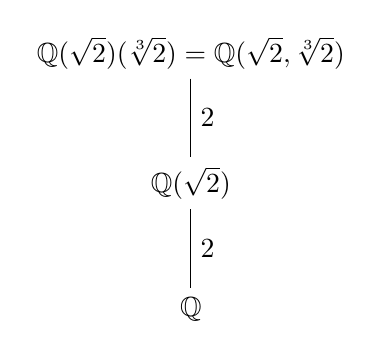
\begin{tikzpicture}
    \node (1) {$\mathbb{Q}(\sqrt{2})(\sqrt[3]{2}) = \mathbb{Q}(\sqrt{2}, \sqrt[3]{2})$};
    \node (2) [below = of 1] {$\mathbb{Q}(\sqrt{2})$};
    \node (3) [below = of 2] {$\mathbb{Q}$};

    \path 
    (1) edge node[right] {2} (2)
    (2) edge node[right] {2} (3);
  \end{tikzpicture}
\end{figure}
thus we have that $[\mathbb{Q}(\sqrt{2}, \sqrt[3]{2}) : \mathbb{Q}(\sqrt{2})] = 3$, and hence $[\mathbb{Q}(\sqrt{2}, \sqrt[3]{2}) : \mathbb{Q}] = 6$. The minimal polynomial of $\sqrt{2} + \sqrt[3]{2}$ has degree dividing 6.

\subparagraph{Example}

The fields of the form $K(\sqrt{a})$ and $K(\sqrt{a}, \sqrt{b})$ for non-square elements $a, b \in K$ are called quadratic\index{quadratic (extension)} and biquadratic\index{biquadratic (extension}) extensions of K.
\begin{figure}[H]
  \centering
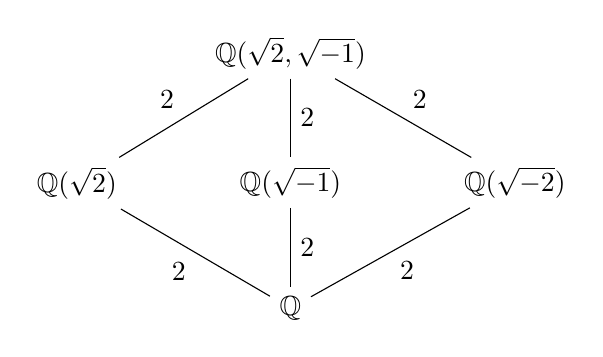
\begin{tikzpicture}
  \node (1) {$\mathbb{Q}(\sqrt{2}, \sqrt{-1})$};
  \node (2) [below left = of 1] {$\mathbb{Q}(\sqrt{2})$};
  \node (3) [below = of 1] {$\mathbb{Q}(\sqrt{-1})$};
  \node (4) [below right = of 1] {$\mathbb{Q}(\sqrt{-2})$};
  \node (5) [below = of 3] {$\mathbb{Q}$};

  \path
  (1) edge node[above left] {2} (2)
  (1) edge node[auto] {2} (3)  
  (1) edge node[auto] {2} (4)
  (2) edge node[below left] {2} (5)
  (3) edge node[auto] {2} (5)
  (4) edge node[auto] {2} (5);
\end{tikzpicture}
\end{figure}
hence $\mathbb{Q}(\sqrt{2}, \sqrt{-1})$ is a finite extension of degree 4, with basis for example $\{1, \sqrt{2}, \sqrt{-1}, \sqrt{-2}\}$.

\subparagraph{Remark}
Finite extensions are algebraic, but there exists infinite algebraic extensions.

\section{K-homomorphisms}

\begin{lemma}\label{lemma:11}
  If L is a field and $\tau : L \rightarrow L'$ be any ring homomorphism (where $L'$ is not a zero ring), then $\tau$ is injective.
\end{lemma}

\begin{proof}
  As $\ker \tau$ is an ideal of L not containing $1 \in L$ (as $\tau(1) = 1$), we have that $\ker \tau = \{0\}$.
\end{proof}

\begin{definition}\label{def:12}
  Let $L/K$, $L'/K$ be two etensions of K. A K-homomorphism\index{K-homomorphism} is a ring homomorphism from L to L' such that $\restr{\tau}{K} = \text{id}$. 

  The set of all K-homomorphisms is denoted by $\text{Hom}_k\left(L, L'\right)$.
\end{definition}

\subparagraph{Note}

All K-homomorphisms are injective. They are sometimes called embedding, and they are K-linear.

We are mainly interested in the set $\homset{L}{\mathbb{C}}$ when $K \subseteq L \subset \mathbb{C}$.

\subparagraph{Example}

\begin{description}
\item[$\mathbb{C}/\mathbb{R}$:] The $\mathbb{R}$-homomorphisms $\tau : \mathbb{C} \rightarrow \mathbb{C}$ are either:
  \begin{equation*}
    z \mapsto z \quad \text{or} \quad z \mapsto \overline{z}
  \end{equation*}
\item [$\mathbb{Q}(\sqrt{2})/\mathbb{Q}$:] The $\mathbb{Q}$-homomorphisms of $\mathbb{Q}(\sqrt{2} \rightarrow \mathbb{C}$. There are two, which verify:
  \begin{IEEEeqnarray*}{rCl}
    \tau_1 &:& \sqrt{2} \mapsto \sqrt{2} \\
    \tau_2 &:& \sqrt{2} \mapsto \sqrt{-2}
  \end{IEEEeqnarray*}
Note that since it is a ring homomorphism, it must send a root of P to a root of $P \in K[X]$.
\item[$\mathbb{Q}(\protect{\sqrt[3]{2}})/\mathbb{Q}$:] Let $\zeta^3=1$, $\zeta \neq 1$, then we have three $\mathbb{Q}$-homomorphisms:
  \begin{IEEEeqnarray*}{rCl}
    \tau_1 &:& \sqrt[3]{2} \mapsto \sqrt[3]{2} \\
    \tau_2 &:& \sqrt[3]{2} \mapsto \zeta\sqrt[3]{2} \\
    \tau_3 &:& \sqrt[3]{2} \mapsto \zeta^2\sqrt[3]{2}
  \end{IEEEeqnarray*}
in this case, the images $\text{Im} \tau_i$ are different subfields of $\mathbb{C}$.
\end{description}

\begin{definition}\label{def:13}
  \begin{enumerate}
  \item For a non-zero $P \in K[X]$ and an extension $L/K$, we denote by $\text{Root}_P(L)$ the set of all roots of P in L.
  \item Let $\alpha \in L$ be algebraic over K. A root of its minimal polynomial $P_\alpha$ over K in L, i.e. an element of $\text{Root}_{P_\alpha}(L)$, is called a conjugate\index{conjugate} of $\alpha$ in L over K.
  \end{enumerate}
\end{definition}

\begin{proposition}[Roots and Homomorphisms I]\label{prop:14}
  Let $F/K$, $E/K$ be two extensions of K and $\alpha \in F$ be algebraic over K. Then, we have a bijection:
  \begin{equation*}
    \homset[K]{K(\alpha)}{E} \rightarrow \rootset[P_\alpha]{E}
  \end{equation*}

In particular, we have that:
\begin{equation*}
  \cardinality{\homset[K]{K_\alpha}{E}} \leq [K(\alpha) : K]
\end{equation*}
\end{proposition}

\begin{proof}
  \begin{enumerate}
  \item We have a well-defined map:
    As $P_\alpha(\alpha) = 0$, and $\tau$ is a ring homomorphism such that $\restr{\tau}{K} = \text{id}$, we have that:
    \begin{equation*}
      P_\alpha(\tau(\alpha)) = \tau{}P_\alpha(\alpha) = 0
    \end{equation*}
(every K-homomorphism sends $\alpha$ to one of its conjugates in K)

\item It is injective:
All elements in $K(\alpha)$ are polynomials in $\alpha$ with coefficients in K, and $\restr{\tau}{K} = \text{id}$, the map is determined by $\tau(\alpha) \in E$.

\item It is surjective:
let $\beta \in \rootset[P_\alpha]{E}$, we define $\tau : K(\alpha) \rightarrow E$ satisfying $\tau(\alpha) = \beta$. Every $x \in K$ is written $x = P(\alpha)$ with $P \in K[X]$ and P is unique up to adding multiples of of $P_\alpha$ (i.e. any other choice of P is of the form $P + P_{\alpha}Q$), and $P_\alpha(\beta) = 0$ hence $P(\beta) \in E$ is well-defined. Hence let $\tau(x) = P(\beta)$, i.e.
\begin{IEEEeqnarray*}{rCl}
  \tau : K(\alpha) & \rightarrow & E \\
         P(\alpha) & \mapsto & P(\beta)
\end{IEEEeqnarray*}
this is a ring homomorphism, and $\restr{\tau}{K} = \text{id}$.

\item $\cardinality{\homset[K]{K(\alpha)}{E}} = \cardinality{\rootset[P_\alpha]{E}} \leq \deg P_\alpha = [K(\alpha) : K]$.
  \end{enumerate}
\end{proof}


%%% Local Variables: 
%%% mode: latex
%%% TeX-master: "Galois"
%%% End: 
\begin{example}[Uniform distribution]
Let $X_1, \dotsc, X_n$ be \iid $\Uniform[0, \theta]$. Let $T = \max X_i$.
$T$ is sufficient for $\theta$. Let $\tilde{\theta} = 2X_1$ be an unbiased estimator for $\theta$.
We have that:
\begin{IEEEeqnarray*}{rCl}
  \EE_\theta[\tilde{\theta} \given T = t] &=& 2\EE_\theta [X_1 \given \max X_i = t] \\
&=& 2 \left\{ \EE_\theta[X_1 \given \max X_i = t, \, X_1 = \max X_i]\PP(X_1 = \max X_i) + \EE_\theta[X_i \given \max X_i = t, \, X_1 \neq \max X_i]\PP(X_1 \neq \max X_i) \right\} \\
&=& 2 \left\{ t \frac{1}{n} + \frac{t}{2}\frac{n-1}{n} \right\} \\
&=& \frac{n+1}{n}t \mpunct{.}
\end{IEEEeqnarray*}
hence $\tilde{\theta} = \frac{n+1}{n} \max X_i$.
\end{example}

\section{Confidence intervals}
\emph{In this section, $\theta$ is scalar.}

\begin{definition}
  A $100\gamma\%$ confidence interval\index{confidence interval} (C.I.) for $\theta$ is a random interval $\left(A(\vec{X}), B(\vec{X})\right)$ such that:
\[
\PP_\theta \left( (\left(A(\vec{X}), B(\vec{X}) \ni \theta \right) \right) = \gamma
\]
no matter what the true value of $\theta$ may be.
\end{definition}

Note that it is the endpoints of the interval that are random.
Interpreting in terms of repeat sampling, if we calculate $\left(A(\vec{x}), B(\vec{x})\right)$ for a large number of samples $\vec{x}$, then approximately $100\gamma\%$ of them will cover the true $\theta$.

\begin{example}[label=ex:confidence_interval]
Let $X_1, \dotsc, X_n$ be \iid $\Normal(\theta, 1)$. Find a $95\%$ confidence interval for $\theta$.

We know $\overline{X} \sim \Normal(\theta, 1/n)$, so we have $\sqrt{n}(\overline{X} - \theta) \sim \Normal(0, 1)$, for all $\theta$. For any $z_1$, $z_2$, such that $\Phi(z_2) - \Phi(z_1) = 0.95$ (where $\Phi$ is the distribution function of $\Normal(0, 1)$), we have:
\[
\PP_\theta \left[ z_1 \leq \sqrt{n}\left(\overline{X} - \theta\right) < z_2 \right] = 0.95 \mpunct{,}
\]
i.e.
\[
\PP_\theta \left[ \overline{X} - \frac{z_2}{\sqrt{n}} < \theta < \overline{X} - \frac{z_1}{\sqrt{n}} \right] = 0.95 \mpunct{.}
\]
so we have that the following is a $95\%$ confidence interval for $\theta$:
\[
\left( \overline{X} - \frac{z_2}{\sqrt{n}}, \, \overline{X} - \frac{z_1}{\sqrt{n}} \right) \mpunct{.}
\]
We know that $\Normal(0, 1)$ is symmetric, so the shortest such interval obtained by using $z_2 = z_{0.025} = -z_1$ where $z_\alpha$ is the upper $100\alpha\%$ of $\Normal(0, 1)$.
\begin{figure}[h]
  \centering

  \begin{tikzpicture}[domain=-3:3,xscale=1.5,yscale=3]
    \draw[help lines, ->] (-3,0)--(3,0);
    \draw[help lines, ->] (0, -1)--(0, 1);

    \draw plot[id=nupp, samples=1000] function{exp(-x**2)/sqrt(2*pi)};

  \end{tikzpicture}

  \caption{$0.025$ Upper percentage point of $\Normal(0, 1)$}
  \label{fig:5.1}
\end{figure}
We find that $z_{0.025} = 1.96$, so the confidence interval is:
\[
\left(\overline{X} - \frac{1.96}{\sqrt{n}}, \overline{X} + \frac{1.96}{\sqrt{n}} \right) \mpunct{.}
\]
\end{example}

\vref{ex:confidence_interval} illustrates a procedure for finding confidence intervals:
\begin{enumerate}
\item Find a quantity $R(\vec{X}, \theta)$ such that the $\PP_\theta$-distribution of $R(\vec{X}, \theta)$ does not depend on $\theta$.
In the previous example, we had that $R(\vec{X}, \theta) = \sqrt{n}(\overline{X} - \theta)$. This is called the pivot\index{pivot}.

\item Write down a probability statement of the form:
\[
\PP_\theta(z_1 < R(\vec{X}, \theta) < z_2) = \gamma \mpunct{.}
\]
Usually, $z_1$, $z_2$ are percentage points.

\item Rearrange the inequalities inside the $\PP_\theta[ \, ]$ to find a confidence interval.
\end{enumerate}

\begin{example}[Normal variables]
Let $X_1, \dotsc, X_n$ be \iid $\Normal(0, \sigma^2)$. Find a $99\%$ confidence interval for $\sigma^2$.
From the probability review, we have that:
\[
\frac{1}{\sigma^2}\sum_{i=1}^n X_i^2 \sim \chi^2_n
\]
Recall $\chi^2_n(\alpha)$ denotes the upper $100\alpha\%$ point of $\chi^2_n$.
So we have that:
\[
\PP_{\sigma^2} \left[ \chi^2_n(0.995) < \frac{1}{\sigma^2}\sum_{i=1}^n X_i^2 < \chi^2_n(0.005) \right] = 0.99 \mpunct{,}
\]
i.e.
\[
\PP_{\sigma^2} \left[ \frac{\sum X_i^2}{\chi^2_n(0.005)} < \sigma^2 < \frac{\sum X_i^2}{\chi^2_n(0.995)} \right] \mpunct{.}
\]
Hence we have that the following is a $99\%$ confidence interval for $\sigma^2$:
\[
\left(\frac{\sum X_i^2}{\chi^2_n(0.005)}, \, \frac{\sum X_i^2}{\chi^2_n(0.995)} \right) \mpunct{.}
\]
If $n = 50$, we get $\chi^2_{50}(0.005) = 79.49$ and $\chi^2_{50} = 27.99$.
\end{example}

\begin{example}[Bernoulli variables]
Let $X_1, \dotsc, X_n$ be \iid $\Bernouilli(p)$ random variables. We know that the \mle of $p$ is $\hat{p} = \overline{X}$.
By the central limit theorem, we have that as $n$ tends to infinity,
\[
\frac{\sqrt{n}(\hat{p})}{\sqrt{p(1^-p)}} \rightarrow \Normal(0, 1) \mpunct{.}
\]
Hence we have that, for $n$ large:
\[
\PP_p \left[ \hat{p} - z_{\frac{1-\gamma}{2}}\sqrt{\frac{p(1-p)}{n}} < p < \hat{p} + z_{\frac{1-\gamma}{2}} \sqrt{\frac{p(1-p)}{n}} \right] \approxeq \gamma \mpunct{.}
\]
But $p$ is unknown, so we approximate $p$ by $\hat{p}$ to give an approximate asymptotic confidence interval for $p$:
\[
\left( \hat{p} - z_{\frac{1-\gamma}{2}}\sqrt{\frac{\hat{p}(1-\hat{p})}{n}}, \, \hat{p} + z_{\frac{1-\gamma}{2}}\sqrt{\frac{\hat{p}(1-\hat{p})}{n}} \right) \mpunct{.}
\]
\end{example}

Note that it is possible to have confidence regions for vector parameters (see example sheet 1). Also, if $\left(A(\vec{X}), B(\vec{X})\right)$ is a $100\gamma\%$ confidence interval for $\theta$ and $\tau(\theta)$ is a monotone increasing function of $\theta$, then $\left(\tau(A(\vec{X})), \tau(B(\vec{X}))\right)$ is a $100\gamma\%$ confidence interval for $\tau(\theta)$.



%%% Local Variables:
%%% mode: latex
%%% TeX-master: "statistics"
%%% End:

\begin{theorem}[Separability]\label{thm:18}
  Let $F/K$ be a finite extensions inside $\mathbb{C}$. Then, we have:
  \begin{equation*}
    \cardinality{\homset{F}{\mathbb{C}}} = [F : K]
  \end{equation*}
\end{theorem}

\begin{proof}
  Let $F = K(\alpha_1, \ldots, \alpha_n)$ (by prop \eqref{prop:10}). If $n = 1$, then this reduces to prop \eqref{prop:15}. Proceed by induction $n$: let $L = K(\alpha_1, \ldots, \alpha_{n-1})$, $F = L(\alpha)$ with $\alpha = \alpha_n$, and consider the restriction map:
  \begin{IEEEeqnarray*}{rCl}
    \homset{F}{\mathbb{C}} &\rightarrow& \homset{L}{\mathbb{C}} \\
    \rho & \mapsto \restr{\rho}{L}
  \end{IEEEeqnarray*}
By proposition \eqref{prop:17}, the inverse image of each $\tau \in \homset{L}{\mathbb{C}}$ has cardinality $\cardinality{\rootset[\tau{}P_\alpha]{\mathbb{C}}}$. Now $\tau{}P_\alpha$ is irreducible in $\tau(L)[X]$ (where $P_\alpha$ is the minimal polynomial of $\alpha$ over L), as it is the image of $P_\alpha \in L[X]$ under the ring isomorphism $L[X] \rightarrow \tau(L)[X]$ extending $\tau : L \rightarrow \tau(L)$. Hence, we have that:
\begin{equation*}
   \cardinality{\rootset[\tau{}P_\alpha]{\mathbb{C}}} = \deg \tau{}P_\alpha = \deg P_\alpha  \qquad \text{(by prop \eqref{prop:15})}
\end{equation*}
but we also have that:
\begin{equation*}
 \deg P_\alpha = [L(\alpha) : L] \qquad \text{(by prop \eqref{prop:7})}
\end{equation*}
thus, we have:
  \begin{IEEEeqnarray*}{rClr}
   \cardinality{\homset{F}{\mathbb{C}}} &=& [L(\alpha) : L] \cdot \cardinality{\homset{L}{\mathbb{C}}}& \\
    &=& [F : L][L : K] & \text{by induction hypothesis} \\
    &=& [F : K] & \text{by tower law} 
  \end{IEEEeqnarray*}
 \end{proof}

We have also proved the following:

\begin{lemma}\label{lemma:19}
  Let $F/K$ be a finite extension inside $\mathbb{C}$ and $K \subseteq L \subseteq F$. Then, the map:
  \begin{IEEEeqnarray*}{rCl}
    \homset{F}{\mathbb{C}} & \rightarrow & \homset{L}{\mathbb{C}} \\
    \rho & \mapsto & \restr{\rho}{L}
  \end{IEEEeqnarray*}
is surjective, i.e. one can extend every K-homomorphism $\tau : L \rightarrow \mathbb{C}$ to F.
\end{lemma}

\begin{theorem}[Primitive element\index{primitive element (theorem)} theorem]\label{thm:20}
  Every finite extensions inside $\mathbb{C}$ is simple.
\end{theorem}

\begin{proof}
  We prove the simplicity of every finite $F/K$ with $\cardinality{K}$ infinite and satisfying the following (in our case, by theorem \eqref{thm:18}):

if $K \subseteq L \subseteq F$, there exists an extension $E/K$ such that $\cardinality{\homset{L}{E}} = [L : K]$.

Let $F = K(\alpha_1, \ldots, \alpha_n)$ (prop. \eqref{prop:10}. We show that $K(\alpha_1, \ldots, \alpha_i)/K$ simple by induction on $i$. By induction hypothesis, suffices to prove that $L = K(\alpha, \beta) \subseteq F$ is simple over K.

For $\gamma \in L$ with $K\subseteq K(\gamma) \subseteq L$, we have:
\begin{equation*}
  \card{\homset{K(\alpha)}{E}} \leq [K(\alpha) : K] \leq [L : K] = \card{\homset{L}{E}}
\end{equation*}
and equality implies $L = K(\alpha)$.

Hence let $d = [L : K]$ and $\homset{L}{E} = \{ \tau_1, \ldots, \tau_d \}$, it suffices to find $\gamma \in L$ such that $\restr{\tau_i}{K(\alpha)}$ are distinct elements of $\homset{K(\alpha)}{E}$, i.e. $\tau_1(\alpha), \ldots, \tau_d(\alpha)$ all distinct.

We try $\gamma$ of the form $\gamma = \alpha{}x + \beta$, with $x \in K$. We need that:
\begin{IEEEeqnarray*}{rCl}
  0 &\neq& \prod_{i \neq j} \left(\tau_i(\gamma) - \tau_j{\gamma}\right) \\
  &=& \prod_{i \neq j}\left[ \left(\tau_i(\alpha)x + \tau_i(\beta)\right) - \left(\tau_j(\alpha)x + \tau_j(\beta)\right)\right] \\
  &=& \prod_{i \neq j}\left(\left(\tau_i(\alpha)-\tau_j(\alpha)\right)x + \left(\tau_i(\beta) - \tau_j(\beta)\right)\right)
\end{IEEEeqnarray*}
So it will do as long as x is not a root of:
\begin{equation*}
  \prod_{i \neq j}\Big(\big(\tau_i(\alpha)-\tau_j(\alpha)\big)X + \big(\tau_i(\beta) - \tau_j(\beta)\big)\Big) \in E[X]
\end{equation*}
which is not identically zero as $\tau_i(\alpha) \neq \tau_j(\alpha)$ or $\tau_i(\beta) \neq \tau_j(\beta)$ for $i \neq j$ (as $\tau_i \neq \tau_j$, and $L = K(\alpha, \beta)$), hence has only finitely many roots. As $\card{K}$ is infinite, we win.
\end{proof}

\subparagraph{Example}

\begin{enumerate}
\item $\mathbb{Q}(\sqrt{2}, \sqrt{3}) = \mathbb{Q}(\sqrt{2} + \sqrt{3})$
\item $\mathbb{Q}(\sqrt{2}, \sqrt[3]{2}) = \mathbb{Q}(\sqrt{2} + \sqrt[3]{2})$
\end{enumerate}

\section{Galois extensions}

\begin{definition}\label{def:21}
  Let $L/K$, $L'/K$ be extensions. If a K-homomorphism $\tau : L \rightarrow L'$ is a bijection (of sets) then $\tau^{-1} : L' \rightarrow L$ is also a K-homomorphism, and we say that $\tau$ is a K-isomorphism\index{K-ismorphism}. A K-isomorphism $L \rightarrow L$ is called a K-automrphism\index{K-automorphism}, and theset of all K-automorphisms of $L$ is a denoted by $\autset{L}$, a subset of $\homset{L}{L}$. It is a group under composition.
\end{definition}

\begin{lemma}
  \label{lemma:22}
  \begin{enumerate}
  \item If there is a K-homomorphism $\tau : L \rightarrow L'$, then $[L : K] \leq [L' : K]$.
  \item If $[L : K] = [L' : K] < \infty$, then every $\tau \in \homset{L}{L'}$ is a K-isomorphism. In particular, $\homset{L}{L} = \autset{L}$ for finite $L/K$.
  \item If $L/K$ is a finite extension inside $\mathbb{C}$, then $\card{\autset{L}} \leq [L : K]$
  \end{enumerate}
\end{lemma}

\begin{proof}
  Recall that K-homomorphisms are injective (lemma \eqref{lemma:11}). 

  Let $V$, $V'$ be vector spaces over K. If there exists K-linear injective maps $V \rightarrow V'$ then $\dim_K \leq \dim_K V'$. An injective K-linear map $V \rightarrow V'$ is bijective if $\dim_K V = \dim_K V' < \infty$ by rank-nullity. This proves the first two claims.

Now, consider:
\begin{equation*}
  \autset{L} = \homset{L}{L} \subseteq \homset{L}{\mathbb{C}}
\end{equation*}
but we have that $\card{\homset{L}{\mathbb{C}}} = [L : K]$.
\end{proof}

\begin{definition}
  \label{def:23}
  A finite extension $L/K$ is called Galois\index{Galois} if:
  \begin{equation*}
    \card{\autset{L}} = [L : K]
  \end{equation*}
\end{definition}
In this case $\autset{K}$ is called the Galois group\index{Galois group} and denoted by $\Gal{L/K}$.

\begin{proposition}
  \label{prop:24}
  Let $L/K$ be a finite extension inside $\mathbb{C}$. The following are equivalent:

  \begin{enumerate}
  \item $L/K$ is Galois \label{prop:24:i}
  \item Every K-homomorphism $\tau : L \rightarrow \mathbb{C}$ maps $L$ into itself. \label{prop:24:ii}
  \item $\forall \alpha \in L$, every conjugate of $\alpha$ over K is in L.\label{prop:24:iii}
  \item $L = K(\alpha_1, \ldots, \alpha_n)/K$, and every conjugate of $\alpha_i (1 \leq i \leq n)$ over K is in L. \label{prop:24:iv}
  \end{enumerate}
\end{proposition}

\begin{proof}
  \begin{description}
  \item[\ref{prop:24:i} $\Leftrightarrow$ \ref{prop:24:iii}] By the proof of lemma \eqref{lemma:22}, we have that:
    \begin{equation*}
      L/K \ \text{Galois} \Leftrightarrow \homset{L}{L} = \homset{L}{\mathbb{C}}
    \end{equation*}
  \end{description}
  
\end{proof}
%%% Local Variables: 
%%% mode: latex
%%% TeX-master: "Galois"
%%% End: 


\section{Rouché's theorem}

\paragraph{Summing series}

Show that
\[
\sum_{n=1}^\infty \frac{1}{n^2} = \frac{\pi^2}{6} \mpunct{.}
\]

Let $f(z) = \frac{\pi \cos (\pi z)}{z^2 \sin (\pi z)}$. $f$ has simple poles at $n \in \ZZ \setminus \{ 0 \}$, and a triple pole at $0$.
The residues of $f$ are as follows. If $n \in \ZZ \setminus \{ 0 \}$, we have that locally $f = h(z)/k(z)$ where $h(n) \neq 0$ and $k$ has a simple $0$.
Hence we have that
\[
\Res_f = \frac{h(n)}{k'(n)} = \frac{1}{n^2}
\]

If $n = 0$, we have that
\begin{IEEEeqnarray*}{rCl}
  \frac{\cos z}{\sin z} &=& (1 - z^2/2 + O(z^4))(z - z^3/3! + O(z^5))^{-1} \\
&=& (1 - z^2/2 + O(z^4))(1 + z/6 + O(z^3)) \\
&=& 1/z - z/3 + O(z^3) \mpunct{.}
\end{IEEEeqnarray*}
Hence we have that $\Res_f (0) = - \pi^2/3$.

With a view to estimate $\abs{f}$, consider the contour $\gamma_N$ the square of side $2N + 1$ centered at the origin.
By the residue theorem, we have that
\[
\int_{\gamma_N} f(z) dz = 2\pi i \left( 2 \sum_{n=1}^N \frac{1}{n^2} - \frac{\pi^2}{3} \right) \mpunct{.}
\]

We aim to show that $\int_{\gamma_N} f(z) dz \rightarrow 0$ as $N \rightarrow \infty$.
We have that

\begin{IEEEeqnarray*}{rCl}
\abs*{\int_{\gamma_N} f(z) dz} &\leq& \sup_{\gamma_N} \abs*{\frac{\pi \cot {\pi z}}{z^2}} \mathop{\ell}{\gamma_N} \\
&\leq& \sup_{\gamma_N} \abs{\cot (\pi z)} \frac{4 (2N + 1) \pi}{(N + 1/2)^2} \mpunct{.}
\end{IEEEeqnarray*}
Suffices to prove that, on $\gamma_N$, $\abs{\cot {\pi z}}$ is bounded.
On vertical sides, $z = \pm (N + 1/2) + iy$ and we have that
\[
\abs{\cot (\pi z)} = \abs{\tan (i \pi y)} = \abs{\tanh (\pi y)} \leq 1 \mpunct{.}
\]
On horizontal sides, we have that $z = x \pm i(N + 1/2)$, and we have that
\begin{IEEEeqnarray*}{rCl}
  \abs{\cot (\pi z)} &=& \abs*{\frac{e^{i \pi (x \pm i (N + 1/2))} + e^{-i \pi (x \pm i (N + 1/2))}}{e^{i \pi (x \pm i (N + 1/2))} - e^{-i \pi (x \pm i (N + 1/2))}}} \\
&\leq& \abs*{\frac{e^{\pi (N + 1/2)} + e^{- \pi ( N + 1/2)}}{e ^{\pi (N + 1/2)} - e^{- \pi (N + 1/2)}}} \\
&=& \coth(N+1/2) \pi \mpunct{.}
\end{IEEEeqnarray*}
However, we have that $\coth$ is a decreasing function for real values, hence this suffices.

\subsection{The argument principle}
Recall that the zeroes and poles of a meromorphic function have a natural multiplicity. If $f(z) = (z -a)^k g(z)$ and $g(a) \neq 0$, $g$ holomorphic near $a$, then $\abs{k}$ is the multiplicity (resp. order) of the zero (resp. pole).

\begin{theorem}[name=Argument principle, key=thm:argument_principle]
 Let $f$ be meromorphic on a domain $U$ and let $\gamma \subseteq U$ be a simple closed curve.
Suppose no zeroes or poles of $f$ lie on $\gamma$, then we have that
\[
\frac{1}{2 \pi i} \int_\gamma \frac{f'(z)}{f(z)} dz = N - P = n(\Gamma, 0)
\]
where $N$ (resp. $P$) are the numbers of zeroes (resp. poles) of $f$ inside $\gamma$ counted with multiplicity, and $\Gamma = f \circ \gamma$.
\end{theorem}

Note that as $z$ moves along a simple contour $\gamma$, then $f(z)$ has a total change in argument of $2 \pi (N - P)$.

\begin{proof}
  Suppose that $f(z) = (z - a)^kg(z)$, as above. Then we have that
\[
\frac{f'(z)}{f(z)} = \frac{k}{z - a} + \frac{g'(z)}{g(z)} \mpunct{.}
\]
Since $g(a) \neq 0$, we see that $\frac{f'(z)}{f(z)}$ has a simple pole at $a$, and moreover the residue is $+k$ if $f$ had a zero of order $k > 0$ and $-k$ if $f$ had a pole of order $k > 0$.
By the residue theorem, we have that
\[
\frac{1}{2 \pi i} \int_{\gamma} \frac{f'(z)}{f(z)} dz = \sum_{a \text{ inside } \gamma} Res_{f'/f}(a) = N - P \mpunct{.}
\]
Note that since $f$ has no zeroes or poles on $\gamma$, the composite $\Gamma = g \circ \gamma$ is a closed curve in $\CC^* = \CC \setminus \{ 0 \}$.
By definition, we have that
\[
n_\Gamma(0) = \frac{1}{2 \pi i}\int_\Gamma \frac{dw}{w} \mpunct{.}
\]
Letting $w = f(z)$, we obtain the 2\textsuperscript{nd} identity of the theorem.
\end{proof}

\begin{corollary}[Rouché's theorem]
  Let $f$, $g$ be holomorphic on a domain $U$.
Let $\gamma$ be a simple closed curve in $U$.
Assume $\abs{f} > \abs{g}$ on $\gamma$.
Then $f$ and $f + g$ have the same number of zeroes inside $\gamma$, when counted with multiplicity.
\end{corollary}

\begin{proof}
  We want to show that $(f + g)/f = 1 + g/f$ has the same number of zeroes as poles (counted with multiplicity) inside $\gamma$.
Remark that $\abs{f} > \abs{g}$ on $\gamma$ implies that neither $f$ nor $f + g$ can vanish on $\gamma$.
Let $h = 1 + g / f$, this has no zeroes nor poles on $\gamma$ so if $N$, $P$ are the number of zeroes and poles of $h$ inside $\gamma$, $N-P = n_{h \circ g}(0)$.
But if $\abs{f} > \abs{g}$, we have that $z \in \gamma$, and $h(z) \in B_1(1) \subseteq \{ z \mid \Re z > 0 \}$.
On this domain, the principal branch of $\log$ and $\mathrm{arg}$ are continuous.
Hence, the winding number $n_{h \circ g}(0) = 0$.
\end{proof}

\paragraph{Example}
Let $P(z) = z^4 + 6z + 3$. On $\abs{z} = 2$, we have that
\[
16 = \abs{z^4} > 15 = 6\abs{z} + 3 \geq \abs{6z + 3} \mpunct{.}
\]
If $z^4 = f$, $6z + 3 = g$, we have that all zeroes of $P$ satisfy $\abs{z} < 2$.
If $\abs{z} = 1$ and $6 \abs{z} > 4 > \abs{z^4 + 3}$, so $P(z)$ and $6z$ have the same number of zeroes inside $\{ \abs{z} < 1 \}$, so $P$ has $3$ roots (with multiplicity) in the annulus $\{ 1 < \abs{z} < 2 \}$.


%%% Local Variables:
%%% mode: latex
%%% TeX-master: "complex_analysis"
%%% End:

\section{Application I : cyclotomics fields}

\begin{definition}
  For a field K and $N \geq 1$. Let $K(\unityroots{N})$ be a splitting field of $X^N - 1$ over K (cyclotomic extension of K), and $\unityroots{N} = \rootset[X^n -1]{K(\unityroots{N})} \subseteq K(\unityroots{N})^\times$, which lies in a finite extension of $\mathbb{Q}$ or $\mathbb{F}_p$ inside $K(\unityroots{N})$. Then $\unityroots{N}$ is a finite multiplicative group, hence cyclic by lemma \ref{lemma:67}. If $(\mchar K, N) = 1$, then $\card{\unityroots{N}} = N$ by \ref{cor:62}, hence there exists a primitive\index{primitive} N-th root of unity, i.e. $\zeta \in \unityroots{N}$ with order N. There are $\card{\multCyclicGp{N}}$ of them, but no canonical choice like $e^{2\pi{}i/N} \in \mathbb{C}$.
\end{definition}

\begin{proposition}
  \label{prop:70}
  Let $(\mchar K, N) = 1$.

  \begin{enumerate}
  \item We can define the N-th cyclotomic polynomial\index{cyclotomic polynomial} $\Phi_N \in \mathbb{Z}[X]$ inductively by:
    \begin{equation*}
      X^N -1 = \prod_{d \mid N} \Phi_d(X)
    \end{equation*}
    where $d$ runs through all positive divisors of $N$. Denoting the image of $\Phi_N$ in $K[X]$ also by $\Phi_N$, we have:
    \begin{equation*}
      \rootset[\Phi_n]{K(\unityroots{N})} = \{ \text{all primitive N-th roots of 1} \} \subseteq \unityroots{N}
    \end{equation*}

  \item $K(\unityroots{N})/K$ is Galois, with an injective group homomorphism:
    \begin{IEEEeqnarray*}{rCl}
      \Gal{K(\unityroots{N})/K} &\hookrightarrow& \multCyclicGp{N} \\
      (\zeta \mapsto \zeta^i \quad \forall \zeta \in \unityroots{N}) &\mapsto& i \mod  N
    \end{IEEEeqnarray*}
    If $[K(\unityroots{N}) : K] = n$, then all irreducible factors of $\Phi_n$ in $K[X]$ have degree n.
  \end{enumerate}
\end{proposition}

\subparagraph{Example}

\begin{enumerate}
\item $\Phi_2(X) = X+1$
\item $\Phi_3(X) = X^2 + X + 1$
\end{enumerate}

\begin{proof}
  \begin{enumerate}
  \item Induction on $N$. By induction hypothesis $\prod_{d \mid N, d < N}\Phi_d(X)$ is in $Z[X]$, and its roots in $K[\unityroots{N}]$ are all the non-primitive N-th roots of 1, all distinct (by corollary \ref{cor:62}). So it divides $X^N-1$ in $K(\unityroots{N})[X]$, and the roots of the quotient $\Phi_N$ are the primitive N-th roots of 1. Now consider $K = \mathbb{Q}$. Then $\Phi_N \in \mathbb{Q}(\unityroots{N})[X]$ is obtained by the division algorithm as the quotient of $X^N-1$ by a monic polynomial in $\mathbb{Z}[X]$, hence $\Phi_N \in \mathbb{Z}[X]$.

  \item Let $[K(\unityroots{N}) : K] = n$ and $\zeta$ be a primitive N-th root of 1. As $K(\unityroots{N}) = K(\zeta)$ and the minimal polynomial $P_\zeta$ has $\deg P_\zeta = n$ distinct roots in $\unityroots{N}$ (by corollary \ref{cor:62}), hence $K(\unityroots{N})/K$ is Galois by proposition \ref{prop:14}. If $\sigma(\zeta)= \zeta^i$, then $\sigma(\zeta^j) = \left(\zeta^i\right)^j = \left(\zeta^j\right)^i$ for all $j$. The map is injective as $i \mod N$ determines $\sigma$ (as we have $K(\unityroots{N}) = K(\zeta)$), and is a group homomorphism as $(\zeta \mapsto \zeta^i) \circ (\zeta \mapsto \zeta^j) = (\zeta \mapsto \zeta^{ij})$. Finally, every irreducible factor of $\Phi_N$ is the minimal polynomial of some primitive N-th root by the first part, hence has degree $[K(\zeta) : K] = n$.
  \end{enumerate}
\end{proof}

\subparagraph{Example}

Recall in $\mathbb{F}_2[X]$:
\begin{IEEEeqnarray*}{rCl}
 X^15-1 &=& (X+1)(X^2+X+1)(X^4+X^3+X^2+X+1)(X^4+X+1)(X^4+X^3+1) \\
       &=& (\Phi_2\mod 2)(\Phi_3\mod 2)(\Phi_5\mod 2)(\Phi_{15}\mod 2)
\end{IEEEeqnarray*}
so $\Phi_{15}\mod 2$ is a product of two irreducible factors. Note that roots of $\Phi_5\mod 2$ are not generators of $\unityroots{15}$, but still generate $\mathbb{F}_{16}/\mathbb{F}_2$.

\subparagraph{Example}

Let $K = \mathbb{F}_q$ and $n\geq 1$. Since $(\finitefield{q^n})^\times = \unityroots{q^n-1}$ we have $\mathbb{F}_{q^n} = \mathbb{F}_q(\unityroots{q^n-1})$ (splitting field of $X^{q^n} - X$ but also of $X^{q^n-1}-1)$. So every finite extension of finite fields is a cyclotomic extension. Note that $(\text{char} K, q^n -1) = 1$. More generally, for $N \geq 1$, prime to $q$, let $n$ be the order of $q \mod N$ in $\Big(\mathbb{Z}/(N)\Big)$. Then by theorem \ref{thm:68} and proposition \ref{prop:70}, we have:
\begin{IEEEeqnarray*}{rCl}
  \Gal{\mathbb{F}_q(\unityroots{N})/\mathbb{F}_q} &\rightarrow& \{1, q, q^2, \ldots, q^{n-1} \} \subseteq \multCyclicGp{N} \\
  (\text{Fr} : x \mapsto x^q) &\mapsto& q \mod N
\end{IEEEeqnarray*}
is an isomorphism, i.e. $\mathbb{F}_q(\unityroots{N}) = \mathbb{F}_{q^n}$, and all irreducible factors of $\Phi_n$ in $\mathbb{F}_q[X]$ have degree $n$. The previous example is $q = 2$, and $N = 5, 15$, $n = 4$.

So we know how $\Phi_N \mod P$ factorizes for $p$ prime to $N$. What about $\text{char} K = 0$? The simplest case $\multCyclicGp{N}$ is cyclic and has generator $p \mod N$ with p prime, then $\Phi_N \mod p$ is irreducible, hence so is $\Phi_N$. But for example for $N = 8$, $\Phi_8 = X^4+1$, $\Phi_8 \mod p$ is reducible for every prime $p$, but $\Phi_8$ is still irreducible in $\mathbb{Z}[X]$.

\begin{theorem}[Gauss irreducibility of cyclotomic polynomials]
  For all $N \geq 1$, the polynomial $\Phi_N$ is irreducible in $\mathbb{Q}[X]$ (hence also in $\mathbb{Z}[X]$ by Gauss's lemma). In other words, the group homomorphism $\Gal{\mathbb{Q}(\unityroots{N})/\mathbb{Q}} \overset{\cong}{\rightarrow} \multCyclicGp{N}$ in proposition \ref{prop:70} is an isomorphism.
\end{theorem}

\begin{proof}
  Suffices to prove that $\Phi_N$ is the minimal polynomial over $\mathbb{Q}$ of every primitive N-th root of 1, i.e. all elements of $\rootset[\Phi_n]{\mathbb{Q}(\unityroots{N})} = \{ \zeta^a \mid a \in \multCyclicGp{N} \}$ are conjugate over $\mathbb{Q}$.

As every $a \in \multCyclicGp{N}$ is some product of $p \mod N$ for primes $p$ not dividing $N$. Suffices to prove that $\zeta^p$ is a conjugate of $\zeta$ over $\mathbb{Q}$ for every $p$ prime to $N$ and every primitive $\zeta$.

Let $P_\zeta$ be the minimal polynomial of $\zeta$ over $\mathbb{Q}$ and $\Phi_N = P_\zeta\cdot{}Q$ in $\mathbb{Q}[X]$. As $\Phi_N$, $P_\zeta$ are monic, so is $Q$, hence $P_\zeta, Q \in \mathbb{Z}[X]$ by Gauss lemma (since $\Phi_N \in \mathbb{Z}[X]$). Suppose $\zeta^p$ is not a root of $P_\zeta$, then it is a root of Q. Then $\zeta$ is a root of $Q(X^p)$, hence $P_\zeta(X) \mid Q(X^p)$ in $\mathbb{Q}[X]$, hence in $\mathbb{Z}[X]$ (division by a monic polynomial). Reducing this modulo p (and writing $\overline{P} = P \mod p$) $\overline{P_\zeta(X)} \mid \overline{Q(X^P)} = (\overline{Q(X)})^p$ in $\mathbb{F}_p[X]$. Thus $\overline{P_\zeta}$, $\overline{Q}$ have common roots in $\mathbb{F}_p(\unityroots{N})$, but contradicts cor \ref{cor:62} since $\overline{\Phi_N} \mid \overline{X^N-1}$.
\end{proof}


%%% Local Variables: 
%%% mode: latex
%%% TeX-master: "Galois"
%%% End: 

%2nd example after prop 70
% X^15-1 = ... = (\Phi_1 \mod 2)(\Phi_3 \mod 2) ...
%                     ===

$\Phi_n \in \mathbb{Z}[X] \text{ irreducible } \leftarrow \Phi_N = P_\zeta\cdot{}Q$

Suffices to prove that $\zeta$ root of $P_\zeta$ implies $z\hatp$ also a root of $P_\zeta$ with $p \nmid N$.
$\zeta$ root of $P_\zeta$, then $\zeta^p$ root of $Q$, hence $\zeta$ root of $Q(X^p)$. Let $\overline{P} = P \mod p$.
Then $\overline{Q(X^p)} = \overline{Q(X)^p}$ in $\finitefield{p}[X]$. Hence $P_\zeta(X) \nmid Q(X^p)$ implies $\overline{P_\zeta}, \overline{Q}$ have a common root in $\finitefield{p}(\unityroots{N})$.

\subparagraph{Remark}

\begin{enumerate}
\item Later we will see another ``mod p proof'', i.e. proving that $\Gal{P}$ for $P \in \mathbb{Q}[X]$ is large by showing $\Gal{P \mod p}$ is large for some $p$. (see theorem \ref{thm:84}).

\item Let $N = 8$, $\zeta = \zeta_8$, $\Phi_8 = (X-\zeta)(X-\zeta^3)(X-\zeta^5)(X-\zeta^7)$. (add figure 1). By building the theory of number fields and reducing $\mathbb{Z}[\zeta]$ modulo $p$ to get $\finitefield{p}(\unityroots{N}) \reverseinclusion \overline{\zeta} = ``\zeta \mod p''$. (in fact, this is a natural way to obtain all finite extensions of $\finitefield{p}$). One sees from the remark after theorem \ref{thm:68} that the factorization of $\overline{\Phi_8} = \Phi_8 \mod p$ in $\finitefield{p}[X]$ is as:
  \begin{description}
  \item[$p \equiv 1 \mod 8$] $\overline{\Phi_8} = (X - \overline{\zeta})(X - \overline{\zeta^3})(X - \overline{\zeta^5})(X - \overline{\zeta^7})$
  \item[$p \equiv 3 \mod 8$] $\overline(\Phi_8) = \left[(X-\overline{\zeta})(X-\overline{\zeta^3})\right]\left[(X-\zeta^5)(X-\zeta^7)\right]$

e.g. $p = 3$, $\Phi_8 \mod 3 = (X^2+X-1)(X^2-X-1)$
  \item[$p \equiv 5 \mod 8$] $\overline(\Phi_8) = \left[(X-\overline{\zeta})(X-\overline{\zeta^5})\right]\left[(X-\overline{\zeta}^3)(X-\overline{\zeta}^7)\right]$

e.g. $p = 5$, $\Phi_8 \mod 5 = (X^2-2)(X^2+2)$
  \item[$p \equiv 7 \mod 8$] \ldots

e.g. $p = 7$, $\Phi_8 \mod 7 = (X^2 + 3X + 1)(X^2-3X+1)$
  \end{description}
which explains why $\Phi_8$ is irreducible in $\mathbb{Q}[X]$: if it were factorized in $\mathbb{Z}[X]$ (say into $(X-\zeta)(X-\zeta^3)$ etc.), every mod $p$ reduction must respect this.

\item Theorem \ref{thm:71} says $\mathbb{Q}(\unityroots{N})/\mathbb{Q}$ has Galois group $\multCyclicGp{N}$, an abelian group of order $\varphi(N) = \{ i \mod N \mid 1 \leq i \leq N, (i, N) = 1 \}$ (Euler's function\index{Euler's function}). If $N = \prod_i p_i^{m_i}$, then $\varphi(N) = \prod_i \varphi(p_i^{m_i})$, and $\phi(p^m) = p^{m-1}(p-1)$ for $p$ prime. Revisit the ruler and compass construction, a regular N-gon, i.e. points in $\mathbb{Q}(\unityroots{N})$, is constructible if and only if $[\mathbb{Q}(\unityroots{N}) : \mathbb{Q}] = \varphi(N)$ is a power of 2, if and only if $N = 2^ap_1p_2\cdots{}p_r$, where $p_i$ are distinct Fermat primes, e.g. $p = 17$ (Gauss, c.f. example sheet 2.10).
(insert figure 2)
Let $\zeta = \zeta_{17}$, and $\alpha = \zeta + \zeta^{16} = 2\cos \frac{2\pi}{17}$, $\alpha' = \zeta^{13} + \zeta^4$ are roots of $X^2 -\beta_1X + \beta_3$, where $\beta = \beta_1 = \zeta + \zeta^{13} + \zeta^{16} + \zeta^4$, and $\beta_2 = \zeta^9 + \zeta^{15} + \zeta^8 + \zeta^2$ are roots pf $X^2  -\gamma{}X �1$, and $\beta_3$, $\beta_4$ are roots of $X^2 -\gamma'X-1$, with $\gamma = \zeta + \zeta^9 + \cdots + \zeta^2$ (8 terms), and $\gamma' = \zeta^3 + \zeta^{10} + \cdots$ (the rest). Hence $\gamma + \gamma' = 1$, $\gamma\gamma' = -4$, thus $\gamma = \frac{-1 + \sqrt{17}}{2}$.
\end{enumerate}

\section{Separability}

\begin{definition}
\label{def:72}
  Let $K$ be a field. A polynomial $P \in K[X]$ is called separable\index{separable} if $\card{\rootset[P]{E}} = \deg P$ (i.e. no multiple root) whenever P splits in an extension $E/K$ (by lemma \ref{lemma:55}, $\card{rootset{E}}$ independent of $E$).
\end{definition}

\begin{lemma}
\label{lemma:73}
\begin{enumerate}
\item Let $L/K$ be an extension. If $P$ is separable and $Q \in L[X]$ divides $P$ in $L[X]$ then $Q$ is separable.
\item $P$ is separable if and only if $P$ and $D(P)$ are coprime in $K[X]$.
\item If $P$ is irreducible, then $P$ is separable if and only if $D(P) \neq 0$, i.e.$P$ is not a polynomial in $X^p$ for $p = \mchar K$. In particular, all irreducible polynomials are separable if $\mchar K = 0$.
\item Suppose $P$ is separable. If $\tau : K \hookrightarrow E$ is a field homomorphism then $\tau{}P \in E[X]$ is separable. In particular, $P$ is separable as a polynomial in $L[X]$ for any extensions $L/K$.
\end{enumerate}
\end{lemma}

\begin{proof}
  \begin{enumerate}
  \item As $P$ has no multiple root when split, neither does $Q$. 
  \item Let E be a splitting field of $P$. If $P$, $D(P)$ are coprime, then $\exists Q, R \in K[X]$ with $PQ + D(P)R = 1$ in $K[X]$ (recall prop \ref{prop:15}), which remains true in $E[X]$, so $P$, $D(P)$ have no common root in E. If $P$ and $D(P)$ had a common factor in $K[X]$, then they have a common root in E, hence a multiple root.
  \item As $\deg D(P) < \deg P$ and $P$ irreducible, $P$ and $D(P)$ are coprime unless $D(P) = 0$. 
  \item $\tau{}P$ and $\tau{}D(P) = D(\tau{}P)$ are coprime in $E[X]$ (send $PQ + D(P)R = 1$ by $\tau$).
  \end{enumerate}
\end{proof}

%%% Local Variables: 
%%% mode: latex
%%% TeX-master: "Galois"
%%% End: 


\printindex

\end{document}
